\clearpage


\section{FEM}

The vector space $\mathbb{V}$ has infinitely many dimensions.
If we choose n independent functions $v_1,\ldots,v_n$,
then the functions $a_1\cdot v_1(x)+\ldots+a_n\cdot v_n(x)$
span an n-dimensional subspace $\mathbb{V}^{(n)}$ of $\mathbb{V}$.
The following holds:\\

$\boxed{\tilde{u}^{(n)}=a_1\cdot v_1(x)+\ldots+a_n\cdot v_n(x)}$
\subsection{The Method of Ritz}
\textbf{Ritz Matrix: }
$R^{(n)}=\begin{bmatrix}
	R_{1,1}& R_{1,2}&\cdots\\
	R_{2,1}& R_{2,2}&\cdots\\
	\vdots & \vdots &\ddots\\
\end{bmatrix}$ \qquad with \qquad $R_{j,k}^{(n)}=\int\limits_{0}^{1}{v_j'(x)\cdot
v_k'(x) dx}$\\
\textbf{Ritz Vector: }
$r^{(n)}=\begin{bmatrix}
	r_1\\
	r_2\\
	\vdots\\
\end{bmatrix}$ \qquad with \qquad $r_{k}^{(n)}=\int\limits_{0}^{1}{f(x)\cdot v_k(x) dx}$\\

\textbf{Solution according to Ritz:}
$R^{(n)}\cdot a=r^{(n)}\qquad \Rightarrow \qquad a=\left\{R^{(n)}\right\}^{-1}\cdot r^{(n)}$


\subsection{The Method of Galerkin}
\textbf{Galerkin Matrix: }
$G^{(n)}=\begin{bmatrix}
	G_{1,1}& G_{1,2}&\cdots\\
	G_{2,1}& G_{2,2}&\cdots\\
	\vdots & \vdots &\ddots\\
\end{bmatrix}$ \qquad with \qquad $G_{j,k}^{(n)}=\int\limits_{0}^{1}{\underbrace{(v_j''(x))}_{v_j \text{ in Form von DGL!}}\cdot v_k(x) dx}$\\
\textbf{Galerkin Vector: }
$g^{(n)}=\begin{bmatrix}
	g_1\\
	g_2\\
	\vdots\\
\end{bmatrix}$ \qquad with \qquad $g_{k}^{(n)}=\int\limits_{0}^{1}{f(x)\cdot v_k(x) dx}$\\

\textbf{Solution according to Galerkin:} $G^{(n)}\cdot a+g^{(n)}=0\qquad \Rightarrow
\qquad a=\textcolor{red}{\mathbf{-}}\left\{G^{(n)}\right\}^{-1}\cdot g^{(n)}$ \quad according to Ritz $G^{(n)} = -R^{(n)} \quad g^{(n)} = r^{(n)}$\\

The above matrix is only valid for the PDE $-u''(x) = f(x)$ with the ansatz
$\tilde{u}(x) = a_1 \cdot v_1(x) + a_2 \cdot v_2(x)$.
Otherwise, a system of equations for $v_k$ = $v_1$ and $v_2$ must be established
(example for ODE: $u''(x) + u(x) + x = 0$):\\

$\int\limits_{0}^{1}{(a_1 \cdot v_1''(x) + a_2 \cdot v_2''(x) + a_1 \cdot
v_1(x) + a_2 \cdot v_2(x) + x) \cdot v_k(x) dx} = 0
\rightarrow G_{j,k}^{(n)}=\int\limits_{0}^{1}(v_j''(x) + v_j(x))\cdot v_k(x) dx$


\subsection{Weighted Residuals}
Weighting functions: $\{w_1(x),\ldots,w_n(x)\}$

\textbf{Matrix (weighted residuals): }
$M^{(n)}=\begin{bmatrix}
	M_{1,1}& M_{1,2}&\cdots\\
	M_{2,1}& M_{2,2}&\cdots\\
	\vdots & \vdots &\ddots\\
\end{bmatrix}$ \qquad with \qquad $M_{j,k}^{(n)}=\int\limits_{0}^{1}{v_j''(x)\cdot w_k(x) dx}$\\
\textbf{Vector (weighted residuals): }
$m^{(n)}=\begin{bmatrix}
	m_1\\
	m_2\\
	\vdots\\
\end{bmatrix}$ \qquad with \qquad $m_{k}^{(n)}=\int\limits_{0}^{1}{f(x)\cdot w_k(x) dx}$\\

\textbf{Solution of the weighted residuals:}
$M^{(n)}\cdot a+m^{(n)}=0\qquad \Rightarrow \qquad a=\textcolor{red}{\mathbf{-}}\left\{M^{(n)}\right\}^{-1}\cdot m^{(n)}$

\subsection{Point Collocation}
In the context of point collocation (individual points must match between the true result and the approximation),
$n$ support points are chosen in the interval $[0,1]$.
$\begin{bmatrix}
	v_1''(x_1)& v_2''(x_1)&\cdots\\
	v_1''(x_2)& v_2''(x_2)&\cdots\\
	\vdots& \vdots&\ddots
\end{bmatrix}\cdot
\begin{bmatrix}
a_1\\
a_2\\
\vdots
\end{bmatrix}
=\begin{bmatrix}
-f(x_1)\\
-f(x_2)\\
\vdots
\end{bmatrix}$\qquad Solve the system of equations for a\\

The above matrix is only valid for the PDE $-u''(x) = f(x)$ with the ansatz
$\tilde{u}(x) = a_1 \cdot v_1(x) + a_2 \cdot v_2(x)$. Otherwise, the
differential equation (DE) must be formulated with the trial functions, and
substituted at both points to determine $a_1$ and $a_2$:\\
DE: $u''(x) + u(x) = -x$ $\Rightarrow$ Equation at Point 1: $a_1 \cdot
v_1''(x_1) + a_2 \cdot v_2''(x_1) + a_1 \cdot v(x_1) + a_2 \cdot v(x_1) = - x_1$


\subsection{Domain Collocation}
In contrast to point collocation, entire domains (intervals $I_k$) rather than individual points must match.
For $-u''(x) = f(x)$, this system of equations is set up.

$\begin{bmatrix}
	\int_{I_1} v_1'' & \int_{I_1} v_2''& \cdots\\
	\int_{I_2} v_1'' & \int_{I_2} v_2''& \cdots\\
	\vdots& \vdots&\ddots
\end{bmatrix}\cdot
\begin{bmatrix}
a_1\\
a_2\\
\vdots
\end{bmatrix}
=\begin{bmatrix}
-\int_{I_1} f(x)\\
-\int_{I_2} f(x)\\
\vdots
\end{bmatrix}$\qquad Solve the system of equations for a


\subsection{Gauss's Method (MSE)}

\textbf{Gauss Matrix: }
$Q^{(n)}=\begin{bmatrix}
	Q_{1,1}& Q_{1,2}&\cdots\\
	Q_{2,1}& Q_{2,2}&\cdots\\
	\vdots & \vdots &\ddots\\
\end{bmatrix}$ \qquad with \qquad $Q_{j,k}^{(n)}=\int\limits_{0}^{1}{v_j''(x)\cdot v_k''(x) dx}$\\
\textbf{Gauss Vector: }
$q^{(n)}=\begin{bmatrix}
	q_1\\
	q_2\\
	\vdots\\
\end{bmatrix}$ \qquad with \qquad $q_{k}^{(n)}=\int\limits_{0}^{1}{f(x)\cdot v_k''(x) dx}$\\

\textbf{Solution according to Gauss:}
$Q^{(n)}\cdot a+q^{(n)}=0\qquad \Rightarrow \qquad a=\textcolor{red}{\mathbf{-}}\left\{Q^{(n)}\right\}^{-1}\cdot q^{(n)}$

\subsection{Finite Elements}

The discussed methods assume the choice of a set $v_1(x),\ldots,v_n(x)$ of basic functions.
In FEM, local supports (basic functions) are used, which are non-zero only on a small interval.
The advantage of this approach is that in a given region,
only one support influences the approximation function.
The disadvantage lies in the high number of required supports.

\textbf{IMPORTANT:} All methods are presented with a discretization of $h=1/3$.

\subsubsection{Node Variables}
First, on the interval $[0,1]$, $n$ nodes, usually uniformly distributed, are introduced.

\begin{minipage}{11cm}
This divides the interval $[0,1]$ into subintervals (meshes).

For $n=3$:\quad $I_1=[0,1/3]$\quad $I_1=[1/3,2/3]$\quad $I_1=[2/3,1]$

Next, each node $x_k$ is assigned an approximation variable (node variable).

Approximation: \quad $\tilde{u}(0)=a_0$\quad $\tilde{u}(1/3)=a_1$\quad $\tilde{u}(2/3)=a_2$\quad $\tilde{u}(1)=a_3$

Additional conditions:
\begin{tabular}{llll}
$v_0(0)=1$&$v_0(1/3)=0$&$v_0(2/3)=0$&$v_0(1)=0$\\
$v_1(0)=0$&$v_1(1/3)=1$&$v_1(2/3)=0$&$v_1(1)=0$\\
$v_2(0)=0$&$v_2(1/3)=0$&$v_2(2/3)=1$&$v_2(1)=0$\\
$v_3(0)=0$&$v_3(1/3)=0$&$v_3(2/3)=0$&$v_3(1)=1$\\
\end{tabular}
\end{minipage}
\hfill
\begin{minipage}{8cm}
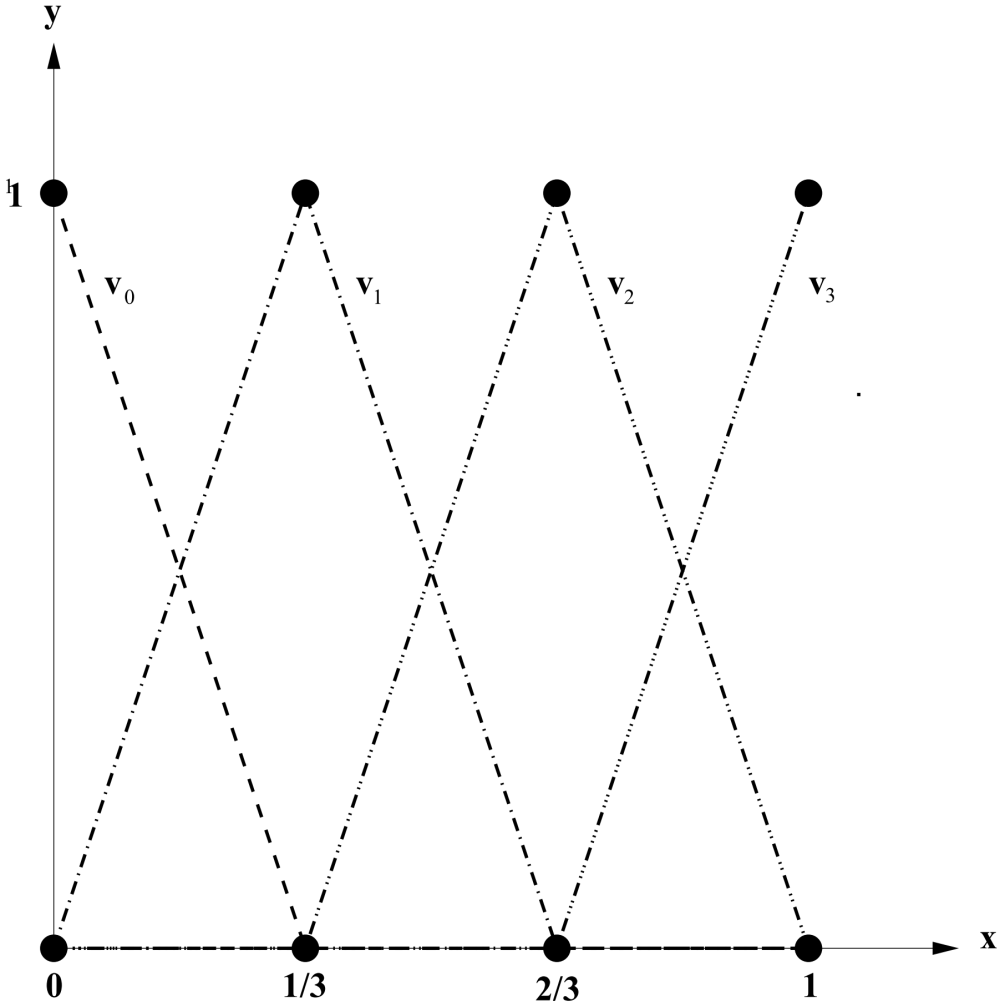
\includegraphics[width=8cm]{Content/02_numerics/Traeger1.png}
\end{minipage}


\subsubsection{Shape Functions}
The local basic functions are intended to be composed of sections of simpler functions, such as polynomials, defined only on a single mesh.\\
Two possible shape functions are, for example, $l_1(x)=1-x$ and $l_2(x)=x$.

\begin{minipage}{8cm}
	\begin{tabular}{lc|c|c}
	$t\in$&$[0,1/3]$&$[1/3,2/3]$&$[2/3,1]$\\
	\hline
	$v_0=$&$1-3x$&$0$&$0$\\
	$v_1=$&$3x$&$2-3x$&$0$\\
	$v_2=$&$0$&$-1+3x$&$3-3x$\\
	$v_3=$&$0$&$0$&$-2+3x$\\
	\end{tabular}
\end{minipage}
\hfill
\begin{minipage}{2cm}
$\Longrightarrow$
\end{minipage}
\hfill
\begin{minipage}{8cm}
	\begin{tabular}{lc|c|c}
	$t\in$&$[0,1/3]$&$[1/3,2/3]$&$[2/3,1]$\\
	\hline
	$v_0=$&$l_1(3x)$&$0$&$0$\\
	$v_1=$&$l_2(3x)$&$l_1(3x-1)$&$0$\\
	$v_2=$&$0$&$l_2(3x-1)$&$l_1(3x-2)$\\
	$v_3=$&$0$&$0$&$l_2(3x-2)$\\
	\end{tabular}
\end{minipage}


\subsubsection{Element Matrices}
In principle, the approximation variable can be determined by any method.
Because in a linear approximation function, the second derivative is trivial ($=0$),
the choice of the Ritz method is enforced.

The integrals are evaluated element-wise:\\

 $\int\limits_{0}^{1}{}=\int\limits_{0}^{1/3}{}+\int\limits_{1/3}^{2/3}{}+\int\limits_{2/3}^{1}{}$\\

 This approach calculates the Ritz matrix for each mesh individually and
 then sums them up to form the global Ritz matrix:\\

\qquad $R^{(4)}=R^{(4,1)}+R^{(4,2)}+R^{(4,3)}=
\begin{bmatrix}
	* & * & 0 & 0\\
	* & * & 0 & 0\\
	0 & 0 & 0 & 0\\
	0 & 0 & 0 & 0\\
\end{bmatrix}+
\begin{bmatrix}
	0 & 0 & 0 & 0\\
	0 & * & * & 0\\
	0 & * & * & 0\\
	0 & 0 & 0 & 0\\
\end{bmatrix}+
\begin{bmatrix}
	0 & 0 & 0 & 0\\
	0 & 0 & 0 & 0\\
	0 & 0 & * & *\\
	0 & 0 & * & *\\
\end{bmatrix}
$\\

The $2\times 2$ matrices marked with $*$ are called mesh matrices:\\

$M^{(4,1)}=M^{(4,2)}=M^{(4,3)}=
\begin{bmatrix}
	* & *\\
	* & *\\
\end{bmatrix}=3\cdot\begin{bmatrix}
	-1 & 1\\
	1 & -1\\
\end{bmatrix}\qquad\Rightarrow\qquad\boxed{M=\frac 1h\cdot
\underset{\text{\textbf{E}: Element matrix}}{\underbrace{\begin{bmatrix}
	-1 & 1\\
	1 & -1\\
\end{bmatrix}}}=\frac 1h\cdot \mathbf{E}}$\\

The element matrix is now inserted into the corresponding Ritz matrix and superimposed.
For the quantization of $h=1/3$, we get:\\

$R^{4}=
\begin{bmatrix}
	-3 & 3 & 0 & 0 \\
	3 & -3-3 & 3 & 0 \\
	0 & 3 & -3-3 & 3 \\
	0 & 0 & 3 & -3 \\
\end{bmatrix}=
\begin{bmatrix}
	-3 & 3 & 0 & 0 \\
	3 & -6 & 3 & 0 \\
	0 & 3 & -6 & 3 \\
	0 & 0 & 3 & -3 \\
\end{bmatrix}$\\

The Ritz vector must be calculated by integration:\\

$r^4=
\begin{bmatrix}
	\int\limits_{0}^{1}{f(x)\cdot v_0(x)dx}\\
	\int\limits_{0}^{1}{f(x)\cdot v_1(x)dx}\\
	\int\limits_{0}^{1}{f(x)\cdot v_2(x)dx}\\
	\int\limits_{0}^{1}{f(x)\cdot v_3(x)dx}\\
\end{bmatrix}$\\

The corresponding Ritz equation system is: $\boxed{R^4\cdot a+r^4=0} \qquad\Rightarrow\qquad a=-\left\{R^4\right\}^{-1}\cdot r^4$\\

\textbf{Initial conditions:} The initial conditions $a_0$ and $a_n$ can be directly substituted.\\


$a_0=10$\qquad$a_3=20$\\

$
	\begin{bmatrix}
		3 & -6 & 3 & 0 \\
		0 & 3 & -6 & 3 \\
	\end{bmatrix}\cdot
	\begin{bmatrix}
		10\\a_1\\a_2\\20
	\end{bmatrix}+r^4=0\qquad\Rightarrow\qquad
	\begin{bmatrix}
		-6 & 3 \\
		 3 & -6 \\
	\end{bmatrix}\cdot
	\begin{bmatrix}
		a_1\\a_2
	\end{bmatrix}+
	\begin{bmatrix}
		30\\60
	\end{bmatrix}+
	r^4=0
$\\

$
	\begin{bmatrix}
			a_1\\a_2
	\end{bmatrix}=
	\begin{bmatrix}
		-6 & 3 \\
	 	 3 & -6 \\
	\end{bmatrix}^{-1}\cdot
	\begin{bmatrix}
		-\left(r^4_1+3\cdot a_0\right)\\
		-\left(r^4_2+3\cdot a_3\right)\\
	\end{bmatrix}
$

\subsubsection{Finite Element Manual Calculation}
\textbf{Problem statement:} $u''(x)+f(x)=0\qquad f(x)=20\qquad u(0)=10\qquad u(1)=20$\\

The approximation should be performed on the \textbf{NON}-uniform intervals:
$[0,1/6]$,\quad $[1/6,1/2]$,\quad $[1/2,1]$\\

The corresponding element matrices E are:\\

$
	\frac{1}{1/6}\begin{bmatrix}
		-1 & 1\\
		1 & -1
	\end{bmatrix}=
	\begin{bmatrix}
			-6 & 6\\
			6 & -6
	\end{bmatrix}\qquad
	\frac{1}{1/2-1/6}\begin{bmatrix}
		-1 & 1\\
		1 & -1
	\end{bmatrix}=
	\begin{bmatrix}
		-3 & 3\\
		3 & -3
	\end{bmatrix}\qquad
	\frac{1}{1-1/2}\begin{bmatrix}
		-1 & 1\\
		1 & -1
	\end{bmatrix}=
	\begin{bmatrix}
		-2 & 2\\
		2 & -2
	\end{bmatrix}
$\\
\\

\begin{minipage}{10cm}
The Ritz Vector and the Ritz Matrix are:\\

$R^n=
\begin{bmatrix}
		-6 & 6 & 0 & 0\\
		6 & -9 & 3 & 0\\
		0 & 3 & -5 & 2\\
		0 & 0 & 2 & -2\\
\end{bmatrix}$

$
r^n=\begin{bmatrix}
		\int\limits_{0}^{1/6}{f(x)\cdot(1-6x)}dx\\
		\int\limits_{0}^{1/6}{f(x)\cdot(6x)}+\int\limits_{1/6}^{3/6}{f(x)\cdot(3/2-3x)}dx\\
		\int\limits_{1/6}^{3/6}{f(x)\cdot(3x-1/2)}+\int\limits_{3/6}^{1}{f(x)\cdot(2-2x)}dx\\
		\int\limits_{1/2}^{1}{f(x)\cdot(2x-1)}dx\\
\end{bmatrix}=
\begin{bmatrix}
	5/3\\
	5\\
	25/3\\
	5
\end{bmatrix}
$\end{minipage}
\hfill
\begin{minipage}{9cm}
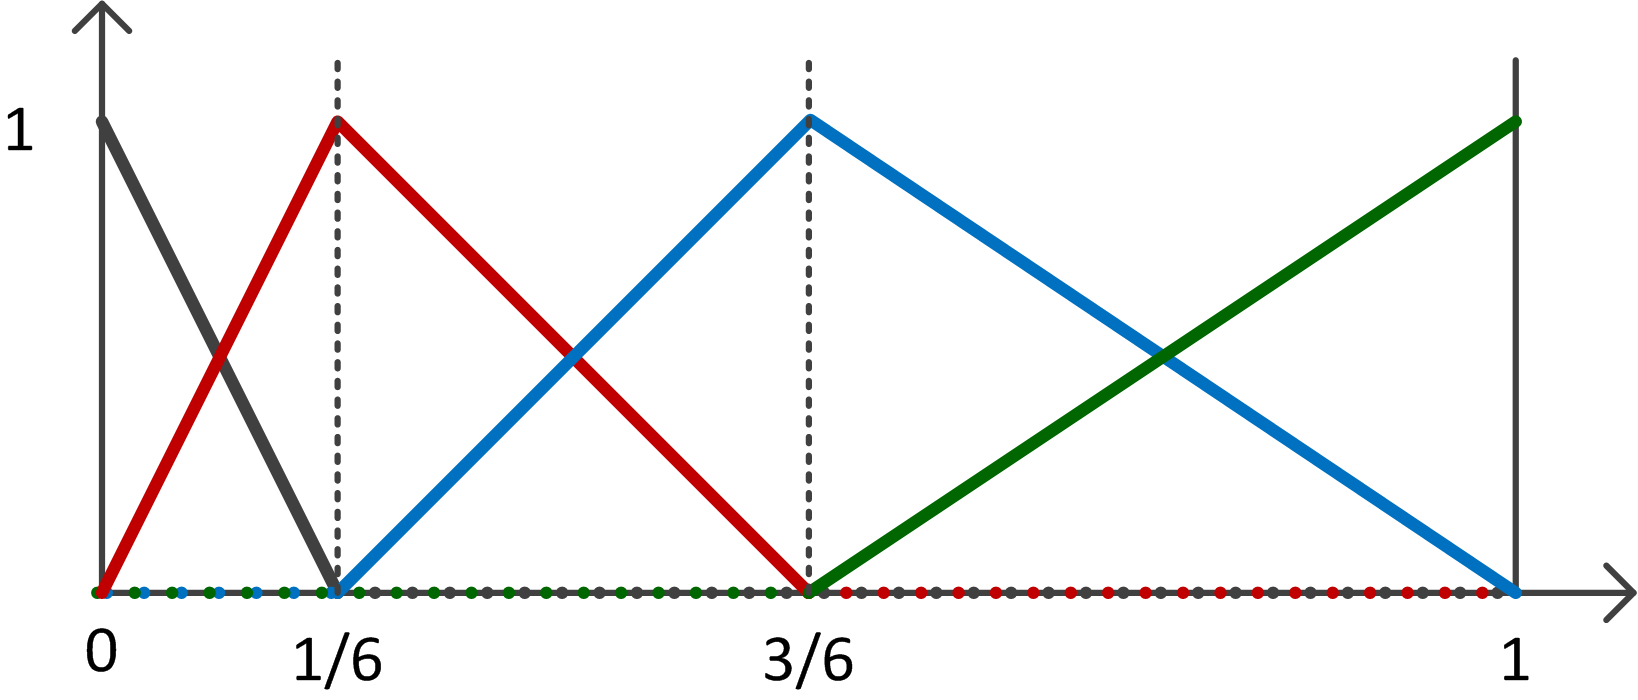
\includegraphics[width=9cm]{Content/02_numerics/FEMHand}
\end{minipage}\\

$R^n\cdot a +r^n=0 \qquad\Rightarrow\qquad
\begin{bmatrix}
	-6 & 6 & 0 & 0\\
	6 & -9 & 3 & 0\\
	0 & 3 & -5 & 2\\
	0 & 0 & 2 & -2\\
\end{bmatrix}\cdot
\begin{bmatrix}
	10\\
	a_1\\
	a_2\\
	20
\end{bmatrix}+
\begin{bmatrix}
	5/3\\
	5\\
	25/3\\
	5
\end{bmatrix}=
\begin{bmatrix}
	0\\
	0\\
	0\\
	0
\end{bmatrix}\qquad\Rightarrow\qquad
\begin{bmatrix}
	6 & -9 & 3 & 0\\
	0 & 3 & -5 & 2\\
\end{bmatrix}\cdot
\begin{bmatrix}
	10\\
	a_1\\
	a_2\\
	20
\end{bmatrix}+
\begin{bmatrix}
	5/3\\
	5\\
	25/3\\
	5
\end{bmatrix}=
\begin{bmatrix}
	0\\
	0\\
	0\\
	0
\end{bmatrix}
$\\
\\

$\qquad\Rightarrow\qquad
\begin{bmatrix}
	-9 & 3\\
	3 & -5\\
\end{bmatrix}\cdot
\begin{bmatrix}
	a_1\\
	a_2\\
\end{bmatrix}+
\begin{bmatrix}
	6\cdot 10\\
	2\cdot 20\\
\end{bmatrix}+
\begin{bmatrix}
	5\\
	25/3\\
\end{bmatrix}
=0\qquad\Rightarrow\qquad
\begin{bmatrix}
	-9 & 3\\
	3 & -5\\
\end{bmatrix}\cdot
\begin{bmatrix}
	a_1\\
	a_2\\
\end{bmatrix}=
\begin{bmatrix}
	-65\\
	-145/3\\
\end{bmatrix}\qquad\Rightarrow\qquad
\begin{bmatrix}
	a_1\\
	a_2\\
\end{bmatrix}=
\begin{bmatrix}
	235/18\\
	35/2\\
\end{bmatrix}
$\\
\\
$
\qquad\Rightarrow\qquad \tilde{u}(x)=10\cdot v_0(x)+\frac{235}{18} v_1(x)+\frac{35}{2}\cdot v_2(x)+20\cdot v_3(x)=
$




\subsubsection{h-Strategy}

The basic idea of the h-strategy is to refine the resolution. In other words,
the mesh width $h$ is reduced. To cover the entire range, more meshes are required.

\subsubsection{p-Strategy}
With the p-strategy, the mesh remains unchanged.
The trial functions should now be composed of higher-order polynomials,
and new nodes and node variables are introduced.\\

\textbf{Problem statement:} $u''(x)+f(x)=0\qquad u(0)=a_0\qquad u(1)=a_6$\\

The approximation should apply to the equally spaced intervals: $[0,1/3]$,\quad $[1/3,2/3]$,\quad $[2/3,1]$\\

\begin{minipage}{4cm}
	Shape functions:\\

	$q_1(x)=(1-x)\cdot(1-2x)$\\
	$q_2(x)=4x\cdot(1-x)$\\
	$q_3(x)=-x\cdot(1-2x)$\\

	Element matrix: $\boxed{E=\frac{1}{3}
	\begin{bmatrix}
		-7& 8 & -1\\
		8& -16& 8\\
		-1& 8& -7
	\end{bmatrix}}$\\
\end{minipage}
\hfill
\begin{minipage}{8cm}
	\begin{tabular}{lc|c|c}
		$x\in$&$[0,1/3]$&$[1/3,2/3]$&$[2/3,1]$\\
		\hline
		$v_0=$&$q_1(3x)$&$0$&$0$\\
		$v_1=$&$q_2(3x)$&$0$&$0$\\
		$v_2=$&$q_3(3x)$&$q_1(3x-1)$&$0$\\
		$v_3=$&$0$&$q_2(3x-1)$&$0$\\
		$v_4=$&$0$&$q_3(3x-1)$&$q_1(3x-2)$\\
		$v_5=$&$0$&$0$&$q_2(3x-2)$\\
		$v_6=$&$0$&$0$&$q_3(3x-2)$\\
	\end{tabular}
\end{minipage}
\hfill
\begin{minipage}{6cm}
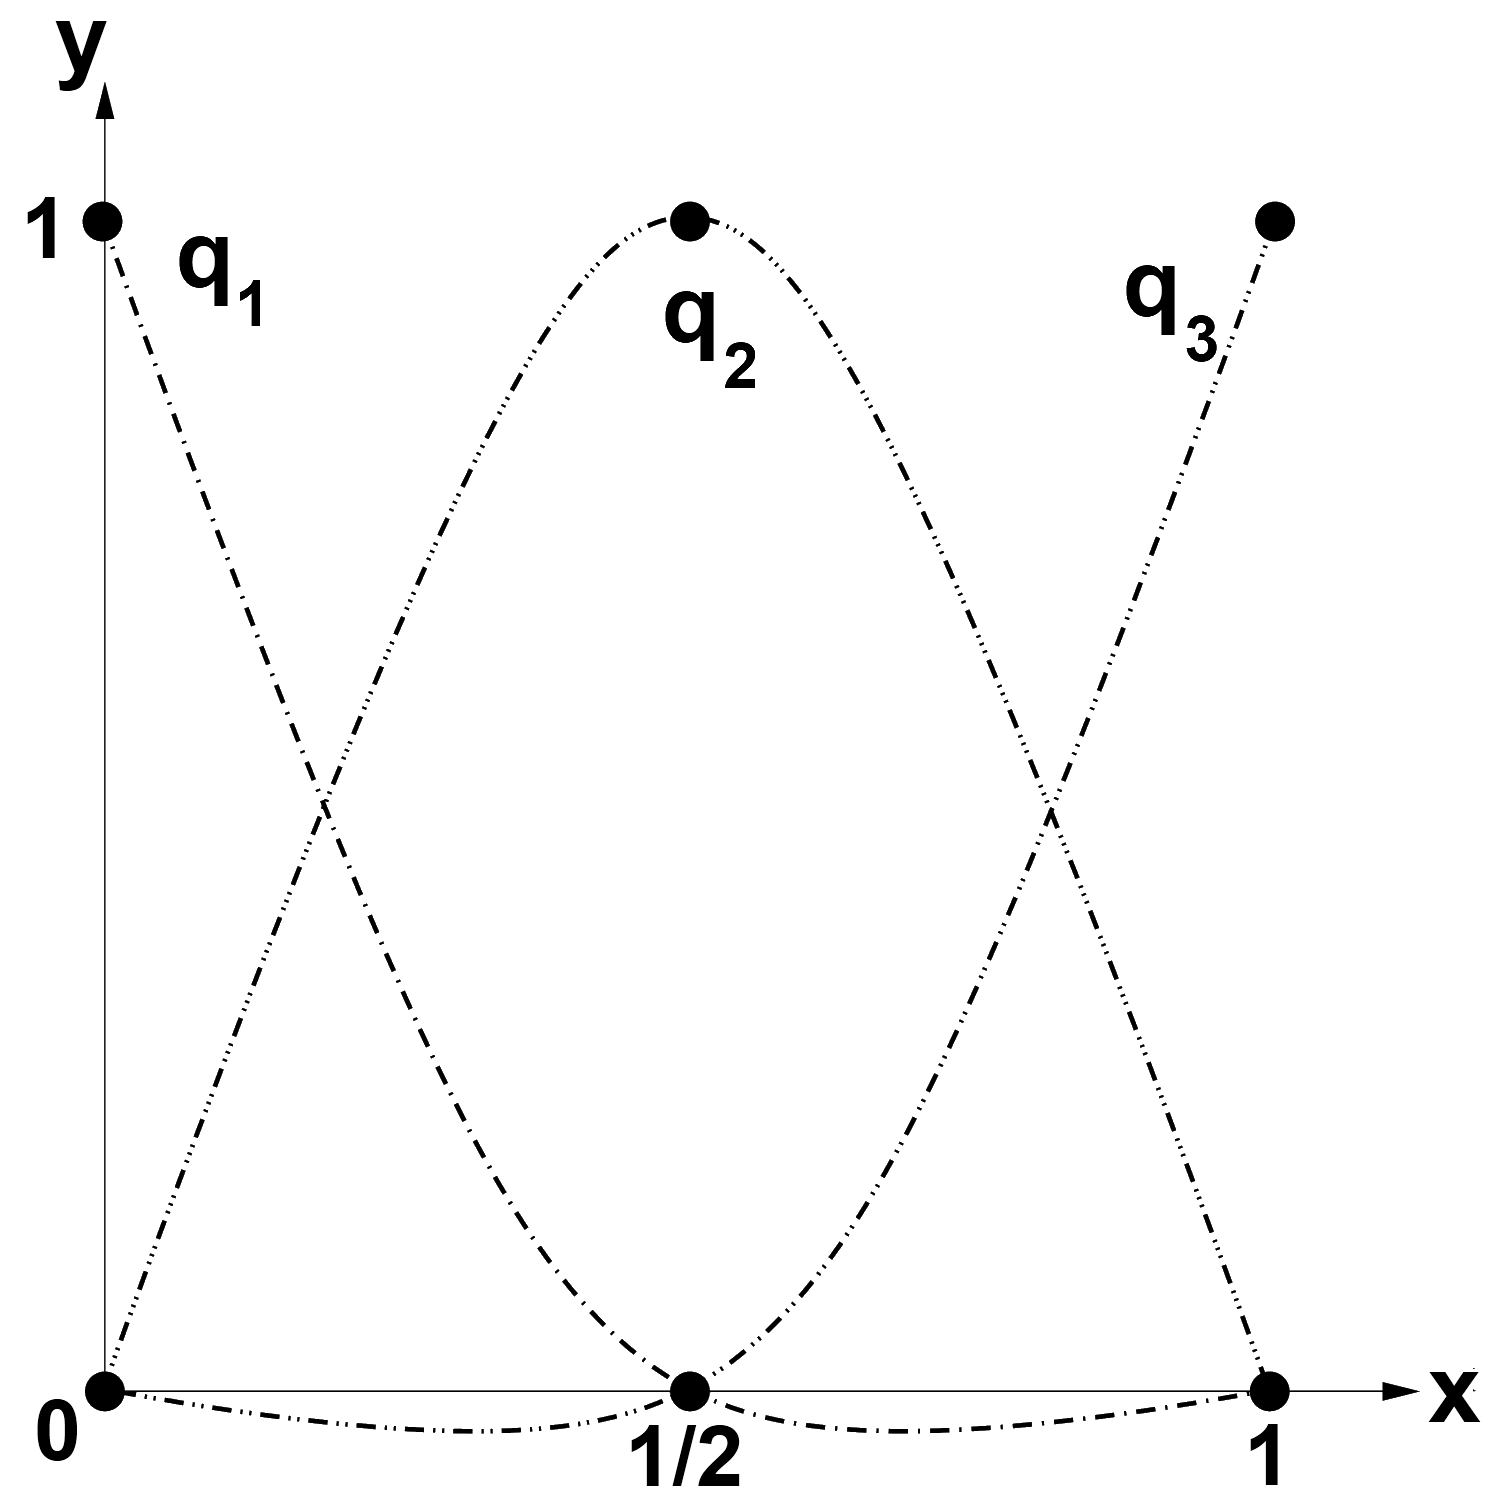
\includegraphics[width=6cm]{Content/02_numerics/FEM2Ord}
\end{minipage}\\

$\underset{\text{Ritz Matrix $R^{(8)}$ for } h=1/3}{\underbrace{\begin{bmatrix}
	-7& 8 & -1& 0& 0& 0& 0\\
	 8& -16& 8& 0& 0& 0& 0\\
	-1& 8& -14& 8& -1& 0& 0\\
	 0& 0& 8& -16& 8& 0& 0\\
	 0& 0& -1& 8& -14& 8& -1\\
	 0& 0& 0& 0& 8& -16& 8\\
	 0& 0& 0& 0& -1& 8& -7
\end{bmatrix}}}\cdot\begin{bmatrix}
	a_0\\
	a_1\\
	a_2\\
	a_3\\
	a_4\\
	a_5\\
	a_6\\
\end{bmatrix}
+\underset{\text{Ritz Vector $r^{(8)}$ for } h=1/3}{\underbrace{\begin{bmatrix}
	\int\limits_{0}^{1}{f(x)\cdot v_0(x)dx}\\
	\int\limits_{0}^{1}{f(x)\cdot v_1(x)dx}\\
	\int\limits_{0}^{1}{f(x)\cdot v_2(x)dx}\\
	\int\limits_{0}^{1}{f(x)\cdot v_3(x)dx}\\
	\int\limits_{0}^{1}{f(x)\cdot v_4(x)dx}\\
	\int\limits_{0}^{1}{f(x)\cdot v_5(x)dx}\\
	\int\limits_{0}^{1}{f(x)\cdot v_6(x)dx}\\
\end{bmatrix}}}=
\begin{bmatrix}
	0\\
	0\\
	0\\
	0\\
	0\\
	0\\
	0\\
	0\\
\end{bmatrix}
$\\

\textbf{Advantage of the p-Strategy over the h-Strategy:}
In both strategies, the dimension of the system matrices increases.
However, there is a justified hope that the increase required to achieve comparable accuracy
is much smaller with the p-strategy than with the h-strategy.

\subsection{Conformity and Completeness}
If the approximate solution must now be differentiable twice,
the approach of the last section is no longer considered conforming.

To ensure single differentiability at the nodes, new basic functions must be found.\\

$\tilde{u}(x)=a_0v_0(x)+a_1v_1(x)+a_2v_2(x)+a_3v_3(x)+\tilde{a}_0\tilde{v}_0(x)+\tilde{a}_1\tilde{v}_1(x)+\tilde{a}_2\tilde{v}_2(x)+\tilde{a}_3\tilde{v}_3(x)$\\

Two basic functions ensure the correct value at the nodes.
Two additional basic functions are needed to ensure the first derivative (slope)
at the transition nodes; they ensure the completeness of the basic functions.
(Without the two additional basic functions, only a slope of zero would be possible at the transition nodes.)

\subsection{Hermite Polynomials of Third Order}
Agreement up to the 1st derivative at the nodes\\

\textbf{Problem statement:} $u''(x)+f(x)=0\qquad u(0)=a_0\qquad u'(0)=\tilde{a}_0 \qquad u(1)=a_3\qquad  u'(1)=\tilde{a}_3$\\

The approximation should apply to the equally spaced intervals: $[0,1/3]$,\quad $[1/3,2/3]$,\quad $[2/3,1]$\\

\begin{minipage}{4cm}
Shape functions:\\
$h_1(x)=2x^3-3x^2+1$\\
$h_2(x)=x^3-2x^2+x$\\
$h_3(x)=-2x^3+3x^2$\\
$h_4(x)=x^3-x^2$
\end{minipage}
\hfill
\begin{minipage}{8cm}
	\begin{tabular}{lc|c|c}
		$x\in$&$[0,1/3]$&$[1/3,2/3]$&$[2/3,1]$\\
		\hline
		$v_0=$&$h_1(3x)$&$0$&$0$\\
		$\tilde{v}_0=$&$\frac 13 h_2(3x)$&$0$&$0$\\
		$v_1=$&$h_3(3x)$&$h_1(3x-1)$&$0$\\
		$\tilde{v}_1=$&$\frac 13 h_4(3x)$&$\frac 13 h_2(3x-1)$&$0$\\
		$v_2=$&$0$&$h_3(3x-1)$&$h_1(3x-2)$\\
		$\tilde{v}_2=$&$0$&$\frac 13 h_4(3x-1)$&$\frac 13 h_2(3x-2)$\\
		$v_3=$&$0$&$0$&$h_3(3x-2)$\\
		$\tilde{v}_3=$&$0$&$0$&$\frac 13 h_2(3x-1)$\\
	\end{tabular}
\end{minipage}
\hfill
\begin{minipage}{6cm}
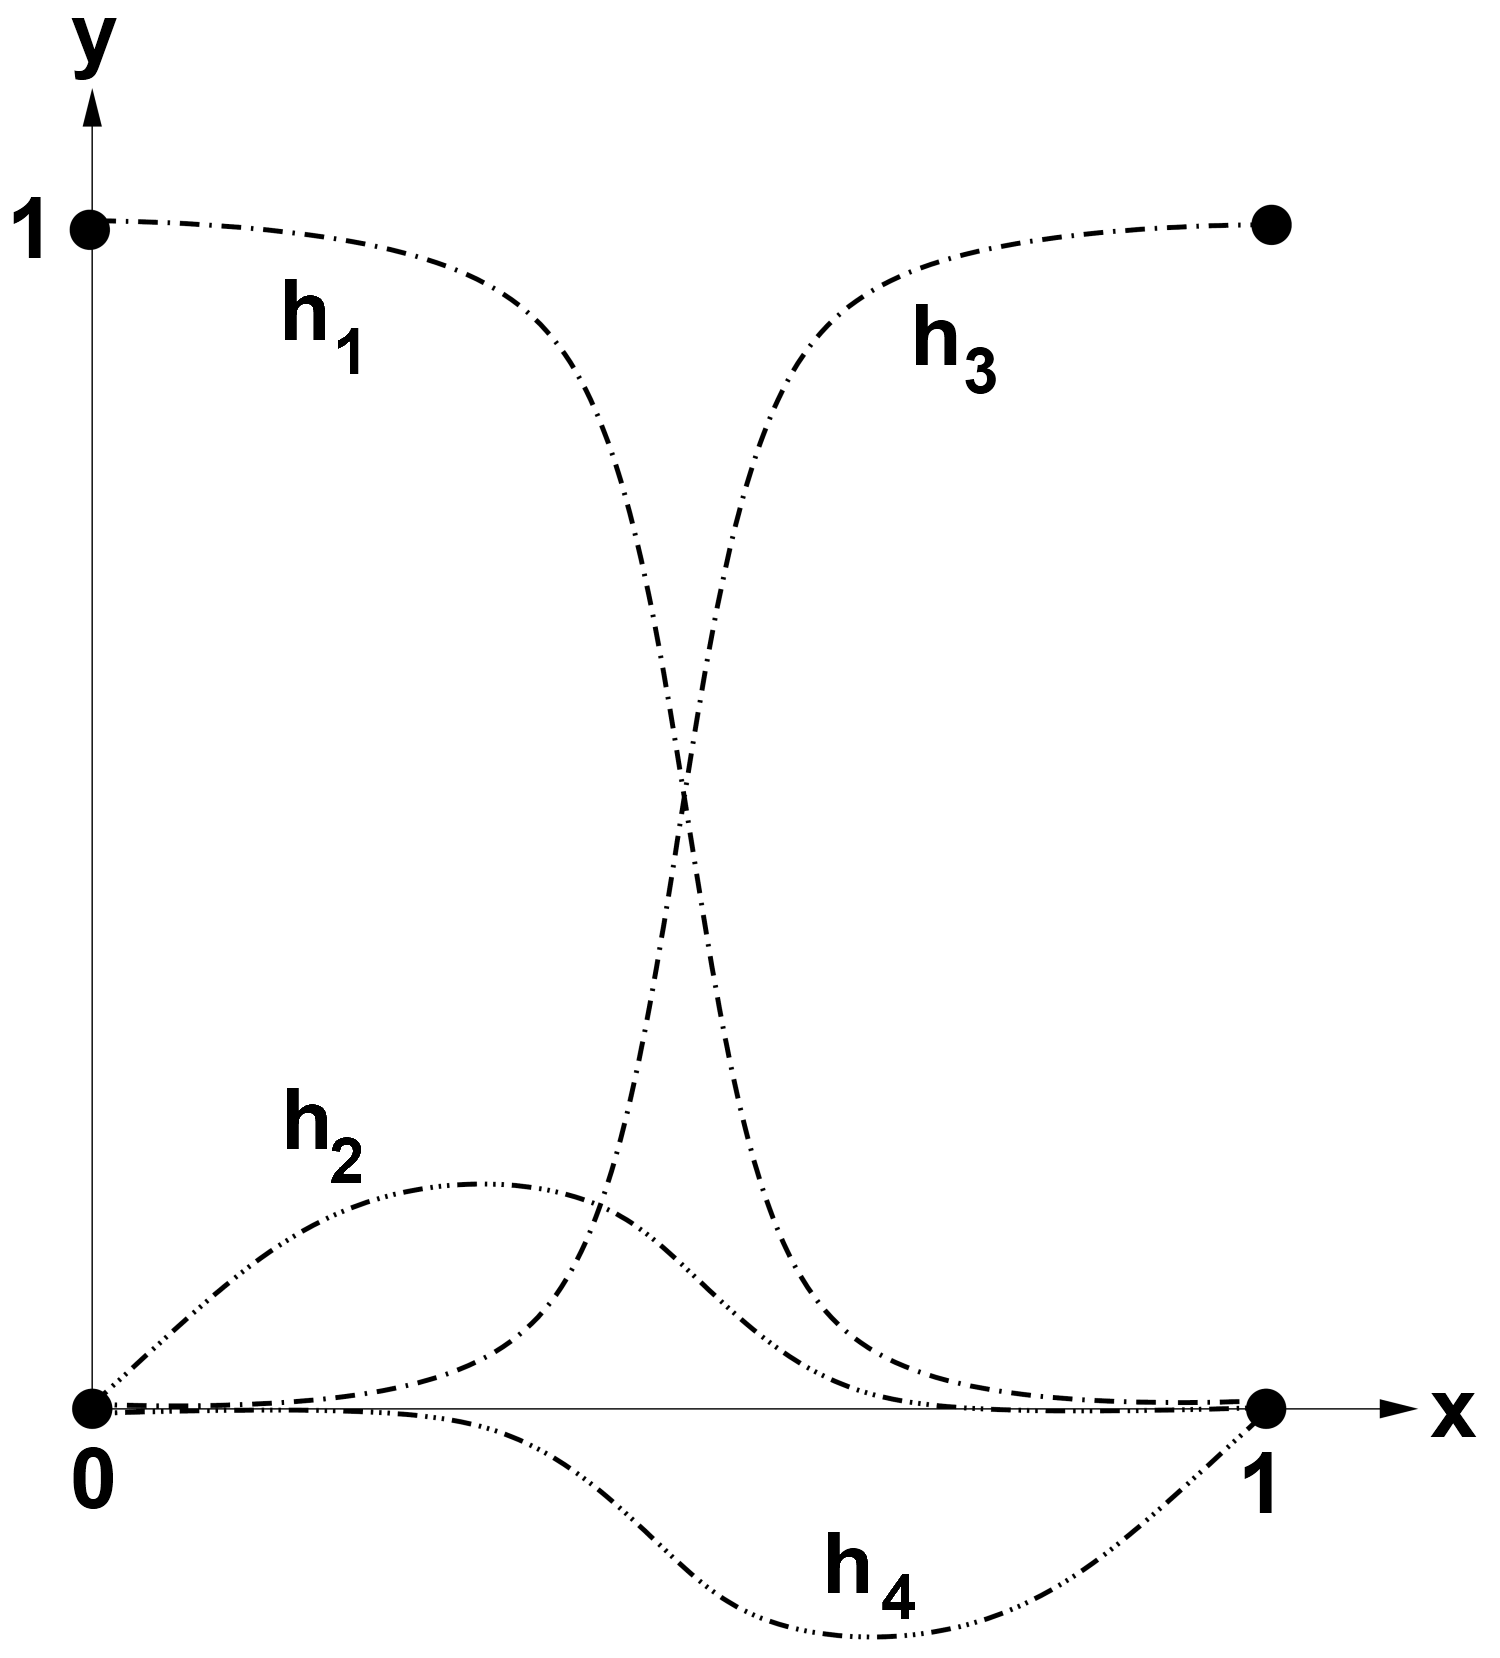
\includegraphics[width=6cm]{Content/02_numerics/FEM3Ord}
\end{minipage}\\
$E=\frac{1}{30}
\begin{bmatrix}
	-36 & -3 & 36 & -3\\
	-3 & -4 & 3 & 1\\
	36 & 3 & -36 & 3\\
	-3 & 1 & 3 & -4\\
\end{bmatrix}\qquad\Rightarrow\qquad
\boxed{M=\frac{1}{30\cdot h}
\begin{bmatrix}
	-36 & -3\cdot h & 36 & -3\cdot h\\
	-3\cdot h & -4\cdot h^2 & 3\cdot h & 1\cdot h^2\\
	36 & 3\cdot h & -36 & 3\cdot h\\
	-3\cdot h & 1\cdot h^2 & 3\cdot h & -4\cdot h^2\\
\end{bmatrix}}$\\
\\


$\underset{\text{Ritz Matrix $R^{(8)}$ for } h=1/3}{\underbrace{\frac{3}{30}\begin{bmatrix}
	-36 & -1 & 36 & -1 & 0  & 0  & 0  & 0 \\
	-1  & -4/9  & 1  & 1/9  & 0  & 0  & 0  & 0\\
	36  & 1  & -72  & 0  & 36  & -1  & 0  & 0\\
	-1  & 1/9  & 0  & -8/9  & 1  & 1/9  & 0  & 0\\
	0  & 0  & 36  & 1  & -72  & 0  & 36  & -1\\
	0  & 0  & -1  & 1/9  & 0  & -8/9  & 1  & 1/9\\
	0  & 0  & 0  & 0  & 36  & 1  & -36  & 1\\
	0  & 0  & 0  & 0  & -1  & 1/9  & 1  & -4/9\\
\end{bmatrix}}}\cdot\begin{bmatrix}
	a_0\\
	\tilde{a}_0\\
	a_1\\
	\tilde{a}_1\\
	a_2\\
	\tilde{a}_2\\
	a_3\\
	\tilde{a}_3\\
\end{bmatrix}
+\underset{\text{Ritz Vector $r^{(8)}$ for } h=1/3}{\underbrace{\begin{bmatrix}
	\int\limits_{0}^{1}{f(x)\cdot v_0(x)dx}\\
	\int\limits_{0}^{1}{f(x)\cdot \tilde{v}_0(x)dx}\\
	\int\limits_{0}^{1}{f(x)\cdot v_1(x)dx}\\
	\int\limits_{0}^{1}{f(x)\cdot \tilde{v}_1(x)dx}\\
	\int\limits_{0}^{1}{f(x)\cdot v_2(x)dx}\\
	\int\limits_{0}^{1}{f(x)\cdot \tilde{v}_2(x)dx}\\
	\int\limits_{0}^{1}{f(x)\cdot v_3(x)dx}\\
	\int\limits_{0}^{1}{f(x)\cdot \tilde{v}_3(x)dx}\\
\end{bmatrix}}}=
\begin{bmatrix}
	0\\
	0\\
	0\\
	0\\
	0\\
	0\\
	0\\
	0\\
\end{bmatrix}
$\\


%\subsection{FEM für parabolische PDEs}
